\chapter{Results}\label{ch:results}\addtocontents{lof}{\protect\contentsline{chapter}{\protect\numberline{\thechapter}Results}{}{}}
% \newthought{Synopsis}\synopsisMethod
The results of the testing of the proof of concept rig are presented in this chapter. The results are presented in a qualitative manner as the rig was not designed to provide quantitative results.
The goal of the testing was to determine if the proof-of-concept rig could simulate the coaptation of the tricuspid valve and the flow of blood through the valve. If the valve leaflets and chordae tendineae could sustain the systolic pressure developed from coaptation, the valve's functionality would be verified for use in the right-heart simulator and later integrated into CroiValve DUO.
\section{Design evaluation and thickness investigation}
The cast valve models showed very good homogeny in thickness, with leaflets thickness having a standard deviation of 0.02mm and an average of 0.40mm

\begin{table}[H]
    \begin{fullwidth}
        \centering
        \footnotesize
        \noindent\makebox[\textwidth]{%
            % \renewcommand{\arraystretch}{1.2}
% \begin{tabular}{p{50pt}|p{75pt}|p{75pt}|p{110pt}|p{55pt}|p{75pt}}
%   \textbf{Authors \& Year} & \textbf{Key Findings}                                                & \textbf{Study Objective}                                            & \textbf{Methodology}                                                                                & \textbf{Relevance to Your Study} & \textbf{Key Learnings}                        \\ \hline
%   Filová et al. 2009       & Calcification of PU in vivo                                          & Overview of tissue-engineered heart valves                          & Meta-Analysis                                                                                       & Material Choice                  & Limited sample size                           \\
%   Baxter et al. 2006       & Flexibility and durability of PU                                     & Overview of synthetic materials in heart valves                     & Tearing energy and crack growth rate tests                                                          & Material Choice                  & Performs even better at elevated temperatures \\
%   Aggarwal et al. 2013     & Converting CT to 3D                                                  & To map patient-specific aortic valves                               & Spline-fitting with mathematic models using echocardiographic images                                & Modelling / Morphology           & Maps microstructure of leaflets               \\
%   Leopaldi et al. 2012     & Comparative data for experimental and simulatory flow-loop           & To develop a flow loop with a porcine heart                         & Endoscopic imaging and hemodynamic measured with ultrasound flowmeter and piezoelectric transducers & Simulator Development            & Compares pressures and flow rates             \\
%   Zilinskas et al. 2022    & Simulator succesfully used for performing valve replacement training & To develop a surgical training simulator using porcine aortic roots & Porcine aortic valve dissected and tether to chamber                                                & Simulator Development            & Demonstrates efficacy of bench-top simulators \\
% \end{tabular}


% \begin{table}
%   \centering
%   \resizebox{\linewidth}{!}{%
\begin{tblr}{
  row{3} = {r},
  row{4} = {r},
  row{5} = {r},
  row{7} = {r},
  row{8} = {r},
  row{9} = {r},
  row{10} = {r},
  row{12} = {r},
  row{13} = {r},
  row{14} = {r},
  row{15} = {r},
  row{16} = {r},
  column{2} = {c},
  cell{1}{1} = {c=2}{},
  cell{2}{1} = {r=4}{},
  cell{2}{3} = {r},
  cell{2}{4} = {r},
  cell{2}{5} = {r},
  cell{6}{1} = {r=5}{},
  cell{6}{3} = {r},
  cell{6}{4} = {r},
  cell{6}{5} = {r},
  cell{11}{1} = {r=6}{},
  cell{11}{3} = {r},
  cell{11}{4} = {r},
  cell{11}{5} = {r},
  cell{17}{1} = {c=2}{},
  cell{18}{1} = {c=2}{},
  vline{3-5} = {1,17-18}{},
  vline{3-5} = {2-16}{},
  hline{2,6,11,17-18} = {-}{},
    }
  Measurement ID     &    & Without Tendineae & With Tendineae & CAD Model   \\
  Posterior          & 1  & 0.38              & 0.45           & 0.40        \\
                     & 2  & 0.38              & 0.41           & 0.41        \\
                     & 3  & 0.39              & 0.41           & 0.41        \\
                     & 4  & 0.39              & 0.50           & 0.40        \\
  Anterior           & 5  & 0.40              & 0.50           & 0.45        \\
                     & 6  & 0.40              & 0.72           & 0.44        \\
                     & 7  & 0.42              & 0.45           & 0.45        \\
                     & 8  & 0.43              & 0.56           & 0.47        \\
                     & 9  & 0.43              & 0.44           & 0.47        \\
  Septal             & 10 & 0.45              & 0.52           & 0.46        \\
                     & 11 & 0.40              & 0.43           & 0.42        \\
                     & 12 & 0.42              & 0.56           & 0.43        \\
                     & 13 & 0.39              & 0.52           & 0.43        \\
                     & 14 & 0.43              & 0.50           & 0.44        \\
                     & 15 & 0.40              & 0.45           & 0.42        \\
  Standard Deviation &    & 0.021104695       & 0.078392654    & 0.023211538 \\
  Average            &    & 0.407333333       & 0.494666667    & 0.433333333
\end{tblr}
% }
% \end{table}}
        \caption{Results of thickness measurements of cast and CAD valve models (mm)}
    \end{fullwidth}
\end{table}

\begin{figure}
    \begin{fullwidth}
        \centering
        \subfloat[Posterior Leaflet]{%
            {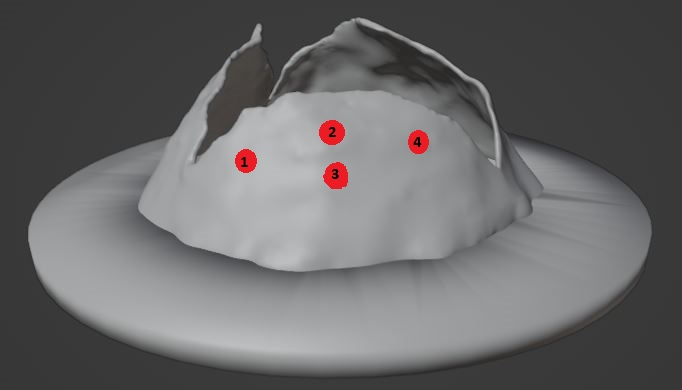
\includegraphics[width=0.30\linewidth]{figures/post}}%
        }\quad
        \subfloat[Anterior Leaflet]{%
            {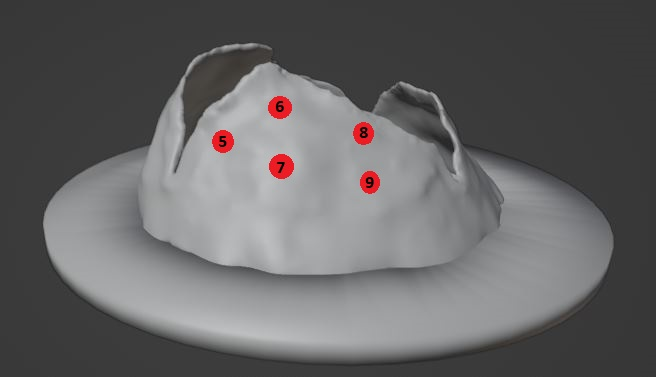
\includegraphics[width=0.30\linewidth]{figures/ant}}
        }
        \quad
        \subfloat[Septal Leaflet]{%
            {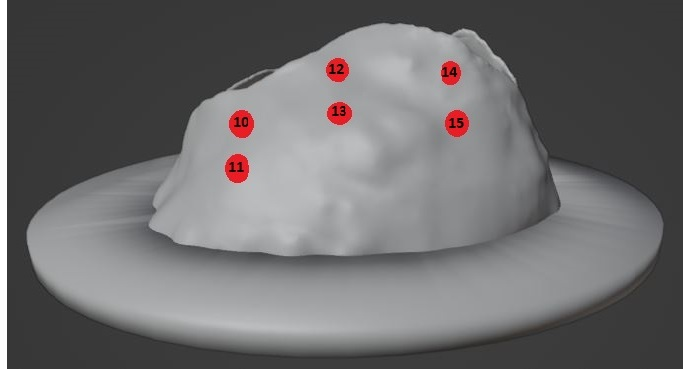
\includegraphics[width=0.30\linewidth]{figures/sep}}
        }
        \caption{Locations of points chosen for thickness measurements on the valve models}
        \label{fig:thicky}
    \end{fullwidth}
\end{figure}
\section{Pilot Tests}
The Teflon tape worked very well where applied; however, the 3D-printed end cap of the core testing chamber leaked a lot even after an attempt to seal with tack. This was due to a misfitting of the O-ring used on the part.

\section{Coaptation Test}
The valve part coapted well, septal and posterior leaflets in particular, the cusp of the anterior leaflet however didnt coapt with either of the adjacent two creating a larger regurgitant orifice than expected. This is likely due to;
\begin{itemize}
    \item The material properties of the \gls{PU} used not being elastic enough.
    \item The thickness of the leaflets being too thick making them less flexible.
    \item The overlapping length of nylon wire on the leaflets making them stiffer.
    \item The natural saddle shape of the valve annulus being flattened off to fit in the seating fixture.
    \item Leaflet length loss from the processing of the valve model.
\end{itemize}

The chordae tendineae held up well under the pressure and prevented the valve from prolapsing. They were tensioned to a point where the valve was allowed to partially prolapse, similar to how native \gls{TV}'s do in regurgitant cases, and an expected degree of prolapse occurred as a result.

During assembly one of the chordae on the posterior leaflet broke leaving just two, however, this didn't affect results.

\begin{figure}
    \begin{fullwidth}
        \centering
        \subfloat[Head-On View]{%
            \href{https://drive.google.com/file/d/1epMX5xH8P03QeNA2DaLtc610iFQK58KK/view?usp=sharing}{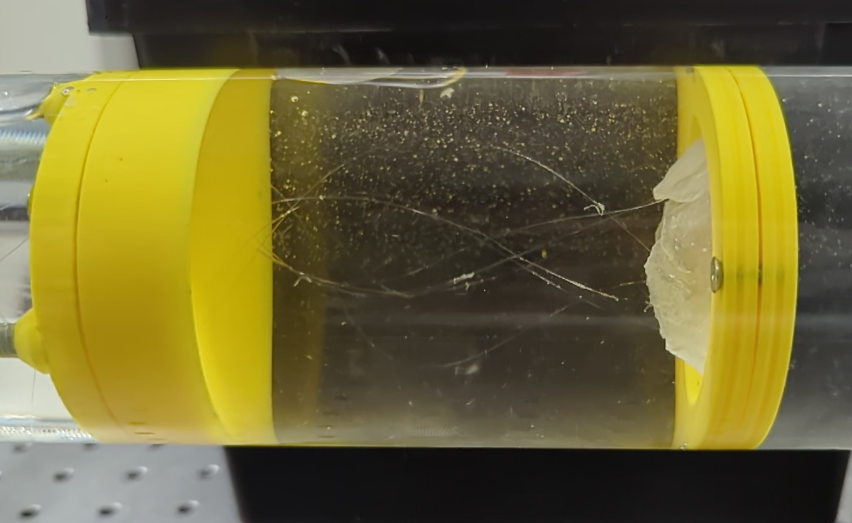
\includegraphics[width=0.45\linewidth]{figures/valverigcloseup}}%
        }\quad
        \subfloat[Oblique View]{%
            \href{https://drive.google.com/file/d/1RXlcIPh9iO5SNXvG8wYL6XBqwaXyd4fS/view?usp=sharing}{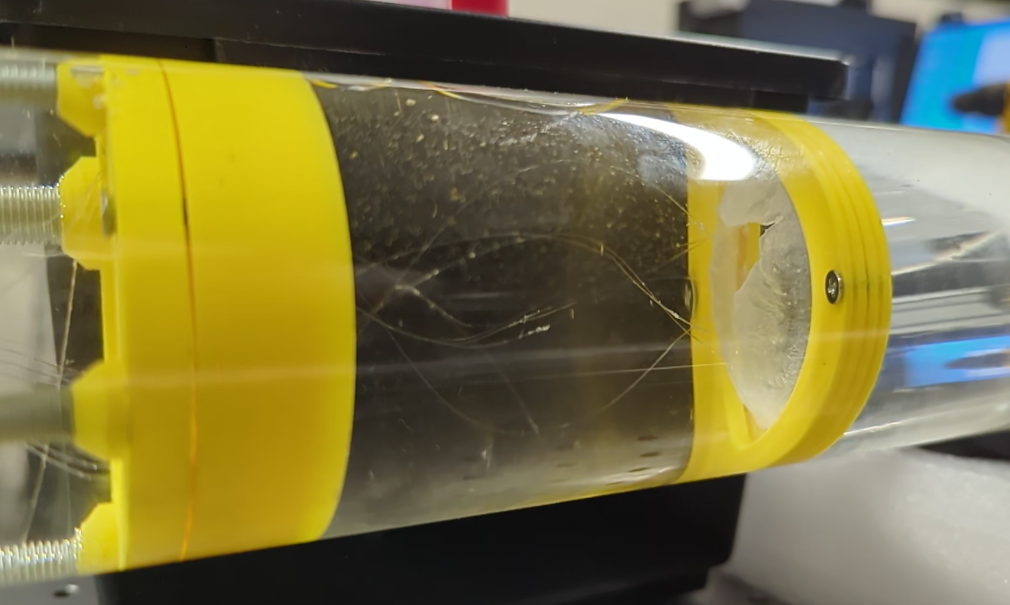
\includegraphics[width=0.45\linewidth]{figures/valverigcloseup2}}
        }
        \caption{Frame from video of valve coapting during testing \textbf{(click to view video)}}
        \label{fig:Videos}
    \end{fullwidth}
\end{figure}